\documentclass[sigconf]{acmart}

\usepackage{booktabs} % For formal tables
\usepackage{cleveref}
\usepackage{xspace}
\usepackage{multirow}
\usepackage{listings}
\usepackage{listingconfig}
\usepackage{enumitem}
\usepackage{graphicx}
\usepackage{caption}
\usepackage{subcaption}
\usepackage{tabularx}

\lstset{language=Racket}

\newcommand{\etal}{\mbox{et al.}\xspace}
\newcommand{\htdp}{\mbox {\sc htdp}\xspace}

\newcommand{\sthree}{\mbox{\sc st1}\xspace}
\newcommand{\sfour}{\mbox{\sc st2}\xspace}
\newcommand{\ssix}{\mbox{\sc st3}\xspace}
\newcommand{\sseven}{\mbox{\sc st4}\xspace}
\newcommand{\sten}{\mbox{\sc st5}\xspace}
\newcommand{\stwelve}{\mbox{\sc st6}\xspace}

\newtheorem{obs}{\textbf{Observation}}

\renewenvironment{quote}
 {\list{}{\leftmargin=0.25in\rightmargin=0.25in}\item[]}
 {\endlist}
 

\begin{document}
\title{Designing a Multi-Faceted SOLO Taxonomy to Track Program Design Skills Through an Entire Course}


\author{Francisco Enrique Vicente Castro}
\affiliation{
  \institution{Worcester Polytechnic Institute}
  \streetaddress{Department of Computer Science}
%   \city{Worcester}
%   \state{Massachusetts}
%   \country{USA}
}
\email{fgcastro@cs.wpi.edu}

\author{Kathi Fisler}
\affiliation{
  \institution{Brown University and WPI}
  \streetaddress{Department of Computer Science}
%   \city{Providence}
%   \state{Rhode Island}
%   \country{USA}
}
\email{kfisler@cs.brown.edu}


% The default list of authors is too long for headers}
\renewcommand{\shortauthors}{Castro and Fisler}


\begin{abstract}

  This paper explores how to assess students' skills in program design and how those skills evolve across an entire CS1 course.  We gathered
  various data from students, including programming samples and
  transcripts from interview and think-aloud sessions. As we coded the
  data, a progression resembling a SOLO taxonomy appeared to emerge
  bottom-up.  As we refined this with top-down perspective from our
  curricular goals, we ended up with a novel multi-faceted SOLO
  taxonomy to track students' progress. We also identified data that
  don't fit a SOLO progression, yet reflect relevant traits and habits
  about design.  In applying our framework, we learned several lessons
  about defining SOLO taxonomies and study protocols that leverage
  them.  The major contributions of this work are (1) a taxonomy
  with separate but inter-related progressions for different design
  skills (that is applied to an entire course rather than a single
  assignment), along with (2) various methodological lessons about
  applying and designing assessments around SOLO taxonomies in this context.

\end{abstract}

\copyrightyear{2017} 
\acmYear{2017} 
\setcopyright{acmlicensed}
\acmConference{Koli Calling 2017}
%\acmBooktitle{17th Koli Calling International Conference on Computing Education Research}
{November 16--19, 2017}{Koli, Finland}\acmPrice{15.00}\acmDOI{10.1145/3141880.3141891}
\acmISBN{978-1-4503-5301-4/17/11}

\fancyhead{}
\settopmatter{printacmref=false, printfolios=false}


% The code below should be generated by the tool at
% http://dl.acm.org/ccs.cfm
% Please copy and paste the code instead of the example below.

\begin{CCSXML}
<ccs2012>
<concept>
<concept_id>10003456.10003457.10003527.10003531.10003533</concept_id>
<concept_desc>Social and professional topics~Computer science education</concept_desc>
<concept_significance>500</concept_significance>
</concept>
<concept>
<concept_id>10003456.10003457.10003527.10003531.10003533.10011595</concept_id>
<concept_desc>Social and professional topics~CS1</concept_desc>
<concept_significance>500</concept_significance>
</concept>
<concept>
<concept_id>10003120.10003121.10003122.10003334</concept_id>
<concept_desc>Human-centered computing~User studies</concept_desc>
<concept_significance>300</concept_significance>
</concept>
</ccs2012>
\end{CCSXML}

\ccsdesc[500]{Social and professional topics~Computer science education}
\ccsdesc[500]{Social and professional topics~CS1}
\ccsdesc[300]{Human-centered computing~User studies}


\keywords{CS1, SOLO taxonomy, program design, qualitative methods}

\maketitle

\section{Introduction}

Introductory computing courses are often designed towards a common
learning outcome: students should be able to develop viable programs
to solve at least small-scale problems. While different
courses may use different programming languages and problem domains,
the underlying program-design skills are fairly common, and include
selecting appropriate language constructs, composing code fragments
for multiple problem tasks, and checking whether the resulting program
satisfies the original problem constraints.

Design skills evolve throughout a course, fostered through repeated
application of language constructs and development of program
schemas. We would expect students to approach program design
differently, and perhaps more systematically, as they gain in
experience and confidence.  Understanding how program-design skills
evolve in novice learners provides valuable input to those who design
curricula and pedagogy.  Such understanding requires both assessments
that explore design skills from various perspectives, but also rubrics
for summarizing design skills across assessments.

This paper reports on the first phase of a study into the evolution of
students' design skills in an introductory CS curriculum. We
interviewed students about their design practices every two weeks
during a 7-week CS1 course.  Two sessions reviewed students' homework
submissions, while the third asked students to solve the Rainfall
problem. We then used open coding on the transcripts to develop a
rubric for assessing the evolution of program-design skills.  What
emerged was a multi-strand SOLO taxonomy. We also identified several factors that are not amenable to a SOLO progression, but suggest potential impact on students' design decisions.  After developing
progressions for individual skill strands, we calibrated across
the strands to give some coherence to each SOLO-level.  Given the
number of component skills that ``program design'' encompasses, we
believe a multi-strand taxonomy offers a more nuanced view of how
design skills develop than more recent efforts to use a single
taxonomy to assess student work along a single dimension.

The main focus of this paper is the design of our multi-strand SOLO
taxonomy, and what we learned from applying it to assess student data
(program solutions and interview/think-aloud data) across an entire course.  Lessons about student design thinking that emerged from using this taxonomy
will be the focus of a different paper. Our main contributions here
are:
\begin{enumerate}
  \item proposing multi-strand SOLO taxonomies
  \item a concrete multi-strand taxonomy that captures aspects of program design beyond coding and algorithm selection
  \item two models for applying the taxonomy across an entire course
  \item methodological lessons about designing such taxonomies and designing
    assessments around those taxonomies
\end{enumerate}

\section{Related Work}

Biggs and Collis proposed the \emph{Structure of Observed Learning Outcomes}
(SOLO) taxonomy model in 1982~\cite{biggs-collis-solo82}.
These taxonomies capture the complexity of learning outcomes, looking
at which aspects of an overall task students have mastered.  Each
taxonomy progresses through five levels of complexity:
\begin{itemize}
\item \emph{Pre-structural}: little to no understanding of the topic
\item \emph{Uni-structural}: understand one aspect of the task
\item \emph{Multi-structural}: understand several aspects of the task,
  but the aspects are understood independently of one another
\item \emph{Relational}: understand several aspects of the task and
  how they inter-operate
\item \emph{Extended Abstract}: can generalize understanding of
  aspects to a new domain
\end{itemize}
\noindent A single taxonomy is intended to detail a progression of
outcomes within a single conceptual task.  Biggs and Collis proposed
the model as assisting in both assessment of student learning and in
creating ``constructive alignment'' between assessments and curricula.

Within computer science, SOLO
taxonomies appear to have first gained traction in the mid 2000s
in the work of CSEd researchers in Australia and New Zealand.
Papers that use SOLO in CS education generally focus on
assessment of student work on a single assessment: researchers identify a
skill that they plan to assess, articulate a SOLO taxonomy relative to
that skill, apply the taxonomy to student work on an assessment (exam
or exercise), and report student performance relative to the
taxonomy. The papers present the final SOLO taxonomy, without
discussing how it was designed. Such papers include Whalley
\etal~\cite{whalley-solo-reading06} (code reading,
comprehension, and summarization), Lister \etal~\cite{lister_not_2006} (code comprehension), Shuhidan \etal~\cite{shuhidan_taxonomic_2009} (writing code to calculate max/min integers), Ginat
\etal~\cite{ginat-solo-algorithmic15} (algorithm design), and Izu
\etal~\cite{izu-code-design-solo16} (code design).

Our work builds on this model in several key ways. Our SOLO
taxonomy is designed to help us track and assess students' progress
across multiple assessments in a (full) course, not just a single
assessment.  As the course naturally targets several skills, our
taxonomy has multiple strands, which we aligned at key points (see
\cref{s:align}). In addition, we detail the process through which we designed our
taxonomy: it results from a combination of bottom-up and top-down analysis
of our data, which grounds our taxonomy in our
larger project from multiple perspectives.

Our taxonomy topics overlap
those of Ginat \etal~\cite{ginat-solo-algorithmic15} and Izu
\etal~\cite{izu-code-design-solo16}.  Ginat's emphasis is on selection
and composition of high-level design patterns.  Task decomposition and
code composition are one of the aspects in our taxonomy, but we frame
the progression differently.  For example, Ginat's unistructural level
captures solutions that translate a specification into a
straightforward use of a single design pattern.  Ours instead assumes
that each problem could have multiple tasks, and calls a solution
unistructural if it maps some single subtask into code (potentially
ignoring other subtasks).  By the relational level, Ginat expects
students to compose plans through interleaving, whereas our taxonomy
expects some composition of code for separate tasks.  In other
writing, Ginat has expressed a preference for interleaved code on the
grounds of efficiency~\cite{muller-ginat-pattern07}.  Our curriculum,
in contrast, does not emphasize efficiency, but teaches students to
think about readability and maintainability as code is adapted to
different contexts.  Thus our two projects have different values
regarding composition skills, which reflect in the different
definitions of our SOLO levels.

Izu \etal (who respond to Ginat \etal) focused on code design
rather than pattern selection and
integration~\cite{izu-code-design-solo16}.  Their taxonomy is in terms
of combining building blocks, which may or may not arise from
previously-learned general patterns.  Our taxonomy has a strand on
writing functions, and like Izu \etal, we look at how students
combine code fragments into solutions.  \Cref{s:align} shows,
however, that our taxonomy shifts from syntactic to semantic understanding
at the boundary of the multistructural and relational levels, whereas
Izu's remains syntactic.  Izu \etal also refer to solving ``the given
task'', whereas for us, identifying individual tasks in the first
place (and mapping them to code) is a key learning objective.  In
general, we believe that having a multi-strand taxonomy lets us
explore inter-related design skills of decomposing problems, mapping
subtasks to code, and composing code.  Both Ginat and Izu conflate or
fix some of these issues.  In addition, neither considers testing,
which we consider an equally-important design skill.

Thompson's SOLO taxonomy for grading programming assignments
(which was also used to design exam questions)
captures multiple
components of activity, but he weaves these into a single strand (that
requires certain behaviors from each
component)~\cite{thompson_holistic_2007}.  For example, the
multistructural level captured students who were ``making the standard
in more than one aspect of the project'', where aspects included code
not crashing, code meeting a baseline of required features, and
following programming and user-interface standards.
We prefer our model
of multiple strands, as it lets us capture when students have made
different levels of progress on different components (whereas Thompson
effectively reduces a students' level to the least level across all
components).
% Meerbaum-Salant \etal combined the SOLO taxonomy with Bloom's taxonomy by
% using a subset of categories from Bloom's as subcategories within the SOLO
% levels (e.g. \emph{Unistructural-Creating, Relational-Creating})
% \cite{meerbaum-salant_learning_2010}. They used this multi-level taxonomy to
% construct questions on various CS concepts (e.g. initialization, loops,
% variables) under each category and evaluated students' performance on these
% questions to assess how well they have ``internalized'' the concepts (i.e.
% answered the question correctly). This served as a scoring rubric to
% potentially point out which concepts students lacked understanding in, but
% does not identify specific progressions around how the CS concepts are learned.
We are not aware of other works that define a family of
inter-related SOLO taxonomies, each tied to the same underlying curriculum.

Some of our interview questions were inspired by work on retrieval of
program schemas~\cite{Pirolli_Anderson_1985,Spohrer_Soloway_1989},
plan composition~\cite{soloway-learning86}, and novice planning
behavior~\cite{Rist_1989,Rist_1991}.  While these works do not suggest
progressions within design practice, they do suggest factors that may
influence program design. Our SOLO strand on task decomposition, in
particular, reflects insights from this work.

\section{Course: \textit{How to Design Programs}}

\begin{figure*}
\begin{lstlisting}
; Problem: Design a function count-votes that consumes a list of names and a specific name,
; and counts how many times the specific name appears in the list of names.

;;; The Data Definition (RECIPE STEP 1)
; A list-of-string is
; - empty, or
; - (cons string list-of-string)

;;; Examples of Data (RECIPE STEP 2)
(define names (cons "pedro" (cons "pedro" (cons "ming" empty))))

;;; The Template (RECIPE STEP 5)
; Traverses the main input type, ignoring other problem-specific parameters.
;   This allows the same template to be reused across multiple functions on the same type.
; The ellipses get filled with details from the specific problem, when the student gets to step 6.
#|
(define (los-func alos)
  (cond [(empty? alos) ...]
        [(cons? alos) ... (first alos)
                      ... (los-func (rest alos)) ...]))
|#

;;; The contract and purpose (RECIPE STEP 3) and final function (RECIPE STEP 6)
; count-votes : list-of-string string -> number
; produces number of times the given string appears in the given list
(define (count-votes alos for-name)
  (cond [(empty? alos) 0]
        [(cons? alos) (cond [(string=? (first alos) for-name)
                             (+ 1 (count-votes (rest alos) for-name))]
                            [else (count-votes (rest alos) for-name)])]))

;;; Test Cases / Examples of Function (RECIPE STEP 4) -- written prior to writing code
(check-expect (count-votes empty "ann") 0)
(check-expect (count-votes names "ann") 0)
(check-expect (count-votes names "pedro") 2)
\end{lstlisting}
\caption{The \htdp recipe steps on a problem to count how many times a given
  string appears in a list. Semicolon is a comment character; vertical
  bars with hash signs create block comments.  Racket naming
  conventions use hyphens to separate words, rather than
  camel casing. \lstinline{cond} is the construct for a multi-armed
  \lstinline{if} statement.  \lstinline{cons} is an operator for
  building lists from an element and an existing list.
  \lstinline{check-expect} captures a test case, with both the
  expression to run and its expected answer.}
\label{f:htdp}
\end{figure*}

\textit{How to Design Programs} (henceforth \htdp) is an introductory
computing curriculum that has been adopted in higher education institutions and some K-12 programs \cite{felleisen_teachscheme!_2004, ramsey_teaching_2014, bieniusa_htdp_2008}. \htdp uses a unique pedagogy for teaching program design through a multi-step process (called the \emph{design recipe}) for designing programs based on the structure of the input data~\cite{fffk:htdp}.  Given a programming problem, students are taught to work through a progression of steps:

\begin{enumerate}
\item Identify and define the structure of the input data.

\item Write (as executable code) examples of the input data.

\item Write the name, input types, and output type (the
  \emph{contract}) for a function that will solve the problem and a
  one-line summary of the program's goal (the \emph{purpose}).

\item Write (as executable code) concrete \emph{examples} (or \emph{test
    cases}) of what the program should produce on specific
  inputs.

\item Write a skeleton of the body of the function that will fully
  traverse the input data (the \emph{template}). The template is
  specific only to the type of input data, not to the computation
  being performed in the given problem.

\item Fill in the template with problem-specific details.

\item Run the function on the tests, adding tests
  as necessary.

\end{enumerate}

\Cref{f:htdp} shows a complete example of the \htdp steps. The code is
written in Racket (a variant of Scheme), the language used in the \htdp textbook~\cite{fffk:htdp}.
The curriculum is particularly well-suited to
functional languages (though some instructors have adapted
it to imperative settings).  It emphasizes data structuring (through
tuples, lists, and trees) more than variations on control flow (beyond
recursion).  While other curricula foster skills such as the selection
of appropriate language constructs, code composition, and checking
program behavior against problem constraints (i.e. testing), these are
embodied either explicitly (e.g. writing tests in \emph{Step 4}) or
implicitly (e.g. necessary construct selection and code composition in
\emph{Step 6}) in the \htdp process.
We are interested in identifying
what skills students draw on or manifest when using the \htdp process.

The steps alternate between thinking abstractly (data types,
contracts, templates) and concretely (examples of data, examples of
program behavior, and completed function code). Each step builds on at
least one previous step. The recipe thus scaffolds the process of
program design, while also serving as a diagnostic for
instructors: if a student is struggling to write a function but can't
describe the input, the student likely
hasn't yet understood the question.
Additionally, the multiple levels of abstraction reflected in the
steps---from contracts, to examples of function behavior (tests),
to the structure of the input data (templates), to the completed code,
gradually provides students more detail for a program solution as they
work through the process. Understanding what relationships students see
between these different levels of abstraction is one of our goals in
studying design process development in \htdp.

An \htdp course shows how to apply the recipe to increasingly rich
data structures: it starts with programs over atomic data (numbers,
strings, images), then progresses to compound data (structs/records),
lists of atomic data, lists of structs, binary trees, and n-ary trees
(mutual recursion). All design steps, including testing and template
design, are re-iterated throughout this progression.  After trees, the
curriculum discusses higher-order functions (maps and filters),
functions that accumulate partial results in parameters, and
introduces stateful variables.  Additional topics are covered in
semester-length \htdp courses; the course used in this study runs on a
shorter calendar, and covers only the listed topics.

\section{Data Collection}
\label{s:data-collect}

\begin{table}
\centering
\caption{Topics and activities for each study session.}
\label{tab:sessions}
\begin{tabular}{|r|l|}
\hline
\multicolumn{2}{|c|}{\textbf{Session 1}}                                                                                                           \\ \hline
\textbf{Topic}      & \begin{tabular}[c]{@{}l@{}}Homework on lists of structs (sum cost of ads \\ for a political candidate)\end{tabular}          \\ \cline{2-2}
\textbf{Activities} & \begin{tabular}[c]{@{}l@{}}(1) Interview on homework solution\\ (2) Compare alternative solutions\end{tabular}               \\ \hline
\multicolumn{2}{|c|}{\textbf{Session 2}}                                                                                                           \\ \hline
\textbf{Topic}      & \begin{tabular}[c]{@{}l@{}}Homework on n-ary trees (check oxygen levels \\ on system of rivers)\end{tabular}                 \\ \cline{2-2}
\textbf{Activities} & \begin{tabular}[c]{@{}l@{}}(1) Interview on homework solution\\ (2) Compare alternative solutions\end{tabular}               \\ \hline
\multicolumn{2}{|c|}{\textbf{Session 3}}                                                                                                           \\ \hline
\textbf{Topic}      & Open coding - Planning (Rainfall)                                                                                            \\ \cline{2-2}
\textbf{Activities} & \begin{tabular}[c]{@{}l@{}}(1) Think-aloud while writing code from scratch\\ (2) Interview on Rainfall solution\end{tabular} \\ \hline
\end{tabular}
\end{table}

Our goal was to study how students evolved in their program-design
skills, as framed by the \htdp design recipe and planning literature,
over the duration of the course.  We were also interested in
identifying underlying factors that might impact how effectively
students were using the recipe.

\subsection{Logistics}

We collected data from study sessions conducted with volunteer CS1 students. Three sessions were conducted individually with each of the volunteers. In sessions 1 and 2, we used an interview protocol to draw out students' knowledge and ideas about their program design process by asking students to describe how they had approached a specific homework problem (which they had recently submitted). We also showed students an alternative solution to what they submitted for homework and asked them to discuss the differences (alternatives might move some
functionality to a helper function, or use an \lstinline{or} statement
in place of an \lstinline{if} statement that returned booleans, for example). In session 3, we gave them a problem to try writing from scratch while talking aloud. After solving the problem, we had them reflect on their work, similar to the activity in sessions 1 and 2 asking students to describe their approach (but without having them compare their work to an alternative implementation). The design of session 3 --- a think-aloud followed by a retrospective interview, was partly adapted from Whalley and Kasto's design \cite{whalley_qualitative_2014} to help clarify interviewer observations during the think-aloud portion in addition to the interview questions used in sessions 1 and 2.
\Cref{tab:sessions} summarizes the topic and activities done in each
session.\footnote{Full homework questions available at:
  https://github.com/franciscastro/koli-2017} \Cref{f:session-ques}
lists the questions through which we asked students to reflect on
their approaches and to compare solutions.

One author conducted all of the sessions, each lasting roughly an
hour. Sessions occurred every two weeks starting after the first exam
(courses at WPI run at intense pace for 7 weeks). Neither
author was instructor for the course. Sessions were individual for
each participant. Each received USD 15 per session and an additional USD 20 upon completing the study. We audio recorded all sessions and collected students' solutions and scratch paper.

\subsection{Problem Selection Rationale}

When selecting problems to include in each session, we wanted problems
that (a) would reflect the various design practices taught in \htdp,
while (b) having at least two identifiable subtasks (so that there
were plausible alternative solutions to discuss).  For the first two
sessions, we discussed problems that involved traversing a data
structure and building up an answer based on data from each element
(each list element or each tree node). In the
first session, a function that computed part of the per-element data
had been assigned as an earlier problem on the same homework.  In the
second session, students were left to consider the per-node task on
their own, without scaffolding from prior problems.  Rainfall \cite{soloway-learning86} (session
3) was different in having multiple traversal-based subtasks (counting, summing, and eliminating some elements): the
default traversal patterns students had learned did not apply naively
to Rainfall, thus letting us see how students employed
their design skills when decomposing richer problems.

The discussions of alternative solutions to problems in sessions 1 and
2 were designed to let us gauge what students notice about solutions:
did they talk only about code, or did they see tasks and structure
within code?  We were curious about which additional criteria (such as
efficiency, readability, or shapes of code) students might bring to
their design work.  Different alternatives for the same problem would
cluster subtasks differently: a function to check whether any list
element met a criterion, for example, could either check the criterion
while traversing the list, or could extract elements that met the
criterion then check whether the list is empty.  Students had been
exposed to functions similar to each subtask in earlier problems, so
this design let us explore what they had picked up from that prior
exposure.

The problems also embodied different suggestions towards testing: the first
session problem looked for a specific name, which suggests
covering data with and without the name; the second had three possible
outputs, each of which should be covered.  Rainfall had some
tests implicit in the problem description (such as those involving
negative numbers), but testing for Rainfall is more subtle as the
position of negative numbers within the list can be important.


% In session 2, one problem was used for the interview and comparison activities. The problem required students to traverse a system of rivers, represented as an n-ary tree, and produce one of three possible results, depending on what the overall state (oxygen level) of the river system was. The problem draws on the use of the \htdp template for traversing trees and here, students use it to traverse each river in the system to check on rivers' oxygen levels. The problem description explicitly states the three possible results, as well as the need for helpers. Some viable solutions include writing a function for each possible outcome, thus traversing the tree multiple times; or extracting the oxygen-level fields (a river is a struct with several fields) into a flat list and using a list template to traverse the flattened data to determine the output. We expected interesting insights about how students approached the problem - whether they saw the instantiation of multiple tree-traversal templates as a viable approach, which subtasks they integrated together, and what their thoughts were about using an intermediate datatype, in this case, one that was likewise different in representation (list) from the original input (tree) to solve the problem, as well as potential tradeoffs this sort of solution would bring up.

% \subsection*{Session 1 Problems}

% \begin{enumerate}
% \item (Compare solutions) Write a function \lstinline{any-ads-for?} that consumes a list of ads and a String representing a product name or politician's name, and produces a Boolean. The function returns \lstinline{true} if the list contains any ads for the given product or politician.
% \item (Talk about solution) Write a function \lstinline{campaign-air-cost} that consumes a list of ads and the name of a politician, and produces the total air-cost of all political ads for that politician.
% \end{enumerate}

% \subsection*{Session 2 Problem}

% \begin{enumerate}
% \item (Talk about solutions; compare solutions) Cold-water fish such as trout and salmon are more vulnerable to low dissolved oxygen (DO) levels than are warm-water fish. Although they can survive for a short time in water with a DO level of less than 5 mg/L, they will die in water below 3 mg/L. Develop a function \lstinline{cold-water-fish-warning} that consumes a river system and produces a string. If all rivers in the system have DO levels at 5mg/L or above, the string produced is ``OK". If any of the rivers in the system have a DO level below 3 mg/L, the function produces the string ``Deadly". Otherwise, the string produced is ``Marginal". You'll need to use helpers here. Think about where you'll want to use the templates.
% \end{enumerate}

% \subsection*{Session 3 Problem}

% \begin{enumerate}
% \item (Think-aloud while programming; talk about solution) Design a program called \lstinline{rainfall} that consumes a list of numbers representing daily rainfall readings. The list may contain the number -999 indicating the end of the data of interest. Produce the average of the non-negative values in the list up to the first -999 (if it shows up). There may be negative numbers other than -999 in the list (representing faulty readings). If you cannot compute the average for whatever reason, return -1.
% \end{enumerate}

\subsection{Participants}

Participants came from a CS1 course at WPI, a selective
STEM-focused university in the USA.
We requested volunteers before the first
exam. Interested students provided information on
their intended major, whether they would take CS2 the following term,
their prior programming experience, programming languages they had used, and a self-evaluation of their performance in the course so far. We separately got their first exam grades from the instructor.

From an initial pool of 15 volunteers, we recruited 13 for the study
(one dropped out before the study began and another wasn't planning to
take CS2---the full study extended over
both courses). We had six males and seven females. In terms of
first-exam performance, 6 students received a grade of A (3 male, 3
female), 3 received a B (2 male, 1 female), and 4 received a C (1
male, 3 female).
% Information about the students is summarized in \cref{tab:students}.

% \begin{table}[]
%   \centering
%   \caption{Student Participants}
%   \label{tab:students}
%   \begin{tabular}{@{}lcccl@{}}
%     \toprule
%     \multicolumn{1}{c}{\multirow{2}{*}{Gender (total)}} & \multicolumn{3}{c}{Exam 1 Grade} & \multicolumn{1}{c}{\multirow{2}{*}{\begin{tabular}[c]{@{}c@{}}Exam 1 {[}Mean, \\ Median, Mode{]}\end{tabular}}} \\ \cmidrule(lr){2-4}
%     \multicolumn{1}{c}{} & \begin{tabular}[c]{@{}c@{}}A \\ (90-100)\end{tabular} & \begin{tabular}[c]{@{}c@{}}B \\ (80-89)\end{tabular} & \begin{tabular}[c]{@{}c@{}}C \\ (65-79)\end{tabular} & \multicolumn{1}{c}{} \\ \cmidrule(r){1-1} \cmidrule(l){5-5}
%     Male (6) & 3 & 2 & 1 & {[}87.67, 89.5, -{]} \\
%     Female (7) & 3 & 1 & 3 & {[}82, 81, -{]} \\
% %    all students (13) & 6 & 3 & 4 & {[}84.62, 89, 90{]} \\
% %    \begin{tabular}[c]{@{}l@{}}Exam 1 {[}Mean, \\ Median, Mode{]}\end{tabular} & \begin{tabular}[c]{@{}c@{}}{[}93.67, \\ 92, 90{]}\end{tabular} & \begin{tabular}[c]{@{}c@{}}{[}85.67, \\ 87, -{]}\end{tabular} & \begin{tabular}[c]{@{}c@{}}{[}70.25, \\ 70, -{]}\end{tabular} &  \\ \bottomrule
% \bottomrule
%   \end{tabular}
% \end{table}

For this phase of the project, we used data from a sample of 6 students to develop the rubric for assessing students' design skills. We randomly selected 2 student volunteers from each of the first-exam grade
bins (for a total of 18 session transcripts).
All 6 students were freshmen (3 male, 3 female), 5 majoring in computer science and one in bioinformatics. Of the 6 randomly selected
students, 1 self-reported having no programming experience prior to
CS1. In terms of self-evaluation of their course performance, 1
reported understanding the topics very well (with an easy time working
on assignments), 4 understood the topics well enough (assignments were
a bit challenging), and 1 found both the topics and course assignments fairly challenging.

\section{Developing an Analysis Framework}

To assess the development of student design skills, we needed to identify which skills students draw on, based on their narratives during the sessions. Developing a rubric for scoring students' design skills was thus the main task for this first phase of the project.

\begin{table*}
\centering
\caption{Emergent themes from open-coding student transcripts.}
\label{tab:emergentthemes}
\subcaption*{(a) SOLO-amenable themes: these became the core skill strands in the multi-strand SOLO taxonomy}
\begin{tabular}{|ll|}
\hline
\textbf{Theme} & \textbf{Description} \\ \hline
\multicolumn{1}{|l|}{\textbf{\begin{tabular}[c]{@{}l@{}}Methodical choice of \\ tests and examples\end{tabular}}} & Knowledge of writing tests; understanding the individual/collective purposes of the tests \\ \hline
\multicolumn{1}{|l|}{\textbf{\begin{tabular}[c]{@{}l@{}}Writing and evaluating \\ function bodies\end{tabular}}} & \begin{tabular}[c]{@{}l@{}}Knowledge of writing functions and the composition of expressions (i.e. built-in/user-defined \\ functions) to build function bodies (i.e. code-level perspective of programs)\end{tabular} \\ \hline
\multicolumn{1}{|l|}{\textbf{\begin{tabular}[c]{@{}l@{}}Decomposing tasks and \\ composing solutions\end{tabular}}} & \begin{tabular}[c]{@{}l@{}}Knowledge of identifying tasks in a given problem, the decompositions of a program into relevant \\tasks, and the composition of solutions to tasks (problem-level perspective of programs)\end{tabular} \\ \hline
\multicolumn{1}{|l|}{\textbf{\begin{tabular}[c]{@{}l@{}}Leverage multiple \\ representations of functions\end{tabular}}} & \begin{tabular}[c]{@{}l@{}}Knowledge of the various representations of functions and how they interact, through the \\ components of the \htdp design recipe\end{tabular} \\ \hline
\end{tabular}
\bigskip
\subcaption*{(b) Non-SOLO themes}
\begin{tabular}{|ll|}
\hline
\textbf{Theme} & \textbf{Description} \\ \hline
\multicolumn{1}{|l|}{\textbf{\begin{tabular}[c]{@{}l@{}}Quality attributes \\ ("ilities")\end{tabular}}} & \begin{tabular}[c]{@{}l@{}}Qualities, properties, or criteria that is expected of or characterizes code or coding practice \\ (e.g. readability and maintainability of code)\end{tabular} \\ \hline
\multicolumn{1}{|l|}{\textbf{Knowledge recalled}} & \begin{tabular}[c]{@{}l@{}}References to knowledge used in programming; this could be course knowledge \\ (i.e. learned from the course) or pre-course knowledge (i.e. learned prior to taking CS1)\end{tabular} \\ \hline
\multicolumn{1}{|l|}{\textbf{Metacognition}} & References to one's cognitive processes or metacognitive behaviors such as self-regulation \\ \hline
\multicolumn{1}{|l|}{\textbf{Value judgments}} & Value judgments towards aspects of the programming process, experience, or learning \\ \hline
\end{tabular}
\end{table*}

\subsection{Identifying Skills and Skill Progressions}
\label{s:solo-themes}

After the first session, we open-coded \cite{charmaz_constructing_2006, kinnunen_phenomenography_2012} the student transcripts from \emph{Session 1} as the other sessions were ongoing. To facilitate this, we literally cut transcript printouts into phrases and iteratively used card sorting\footnote{Card sorting is a method originally employed by psychologists to study how people organize knowledge \cite{wood_card_2008}; it has become a popular user-centered design method for discovering optimal organizations of information for websites or software \cite{wood_card_2008, righi_card_2013}.} to cluster student comments into themes.
Given the questions that we asked students about their work
(\cref{f:session-ques}), which reflected both \htdp and
planning literature, we
expected certain themes to arise in students' responses (e.g., testing,
working with templates, use of learned schemas).  Some themes emerged
independently of the curriculum, while one arose as we sought to align the
emerging codes with the curriculum.
\Cref{tab:emergentthemes} summarizes the resulting themes.

Comments on some themes suggested a \emph{progression within a core skill} (\Cref{tab:emergentthemes}.a) resembling increasing levels of conceptual complexity akin to SOLO levels.
To capture these observed progressions, we defined a SOLO taxonomy for each of these themes by mapping the comments within each theme to a corresponding SOLO level. This produced the multi-strand SOLO taxonomy; each theme identified became a \emph{skill} strand in the overall taxonomy. This was likewise done iteratively to help us refine the concrete definitions of each skill's SOLO level. In one case (\emph{leverage multiple representations of functions}), a SOLO taxonomy arose more top-down, as we tried to make sense of a collection of seemingly related comments within the context of the overall curriculum. We also found other themes that had comments of varying depth, but no core skill that could give rise to a taxonomy (\Cref{tab:emergentthemes}.b --- we discuss these in \cref{sec:open-questions}). \Cref{fig:process} summarizes our iterative open-coding and taxonomy development process. The actual taxonomies for SOLO-amenable themes appear in \cref{tab:solothemes}; we discuss each theme in turn.

\begin{figure}
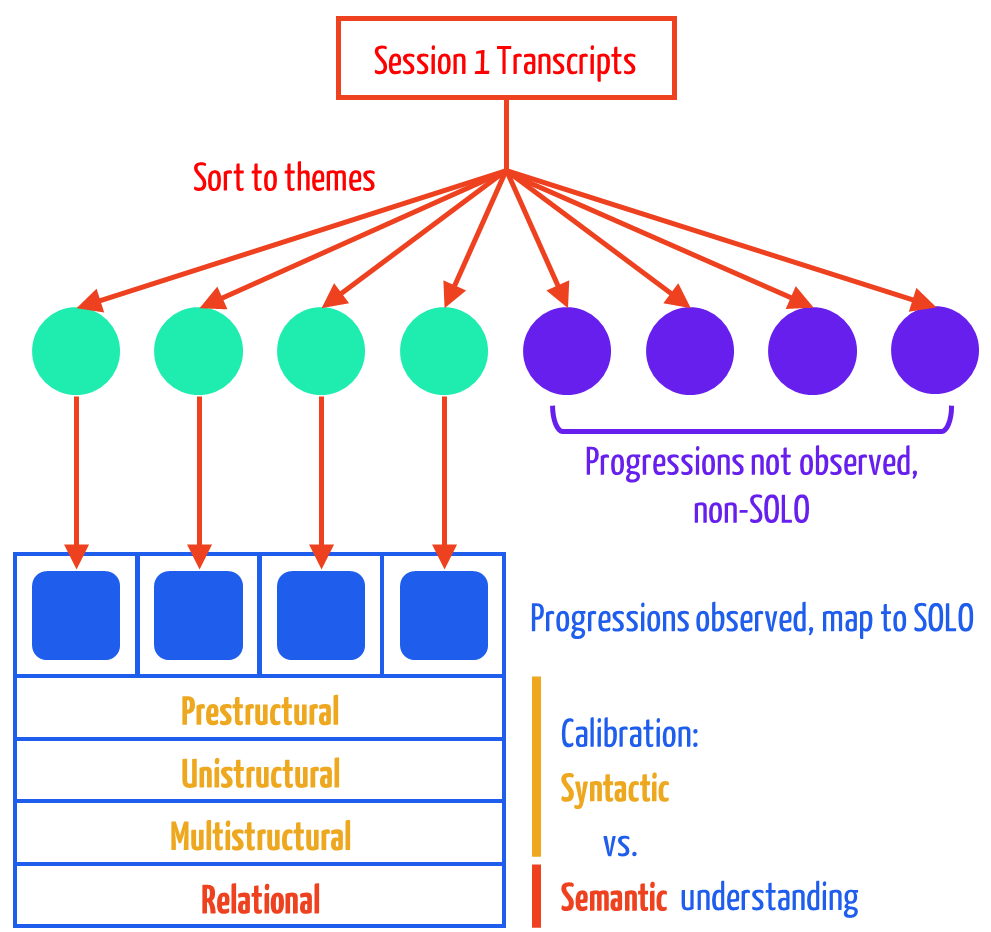
\includegraphics[width=7cm]{process-summary}
\caption{Process summary for developing the multi-faceted SOLO taxonomy. The entire process was done iteratively, with discussions between authors during each iteration refining the themes and descriptions for the taxonomy levels.}
\label{fig:process}
\end{figure}

% \subsection{SOLO-amenable Themes}
% \label{s:solo-themes}

\begin{table*}
\centering
\caption{Multi-strand SOLO taxonomy.  We omit \emph{extended abstract} as none of our students reached that level in this study.}
\label{tab:solothemes}
\begin{tabular}{|l|l|l|l|l|}
\hline
\multicolumn{1}{|c|}{\textbf{SOLO level}} &
\multicolumn{1}{c|}{\textbf{\begin{tabular}[c]{@{}c@{}}Methodical choice of \\ tests and examples\end{tabular}}} &
\multicolumn{1}{c|}{\textbf{\begin{tabular}[c]{@{}c@{}}Writing and evaluating \\ function bodies\end{tabular}}} &
\multicolumn{1}{c|}{\textbf{\begin{tabular}[c]{@{}c@{}}Decomposing tasks and \\ composing solutions\end{tabular}}} &
\multicolumn{1}{c|}{\textbf{\begin{tabular}[c]{@{}c@{}}Leverage multiple repre-\\ sentations of functions\end{tabular}}} \\
\hline
\textbf{Prestructural} &
\begin{tabular}[c]{@{}l@{}}Does not know how to \\ write tests; misses the in-\\ put/output structure of tests\end{tabular} &
\begin{tabular}[c]{@{}l@{}}Does not know how to \\ define a function\end{tabular} &
\begin{tabular}[c]{@{}l@{}}Does not identify relevant\\ tasks for a problem\end{tabular} &
\begin{tabular}[c]{@{}l@{}}Just dives in and writes\\ code; uses only a single \\ representation\end{tabular} \\
\hline
\textbf{Unistructural} &
\begin{tabular}[c]{@{}l@{}}Able to write tests; descrip-\\ tions of tests do not explain\\ the purpose of the test(s);\\ does not express the idea of\\ varying test scenarios\end{tabular} &
\begin{tabular}[c]{@{}l@{}}Able to define functions \\ in a simple context - uses\\ primitive operations on\\ primitive types in a \\ function body\end{tabular} &
\begin{tabular}[c]{@{}l@{}}Able to identify relevant\\ tasks but no reflections of \\ separate tasks when talking\\ about the code\end{tabular} &
\begin{tabular}[c]{@{}l@{}}Blindly follows the design\\ recipe; sees each function\\ representation as indepen-\\ dent of others\end{tabular} \\
\hline
\textbf{Multistructural} &
\begin{tabular}[c]{@{}l@{}}Able to write multiple tests;\\ articulates the purpose of \\ individual tests but does not \\ articulate any relationship \\ between or collective pur-\\ pose for the tests\end{tabular} &
\begin{tabular}[c]{@{}l@{}}Able to define functions\\ whose bodies contain nes-\\ ted non-primitive expres-\\ sions or function calls, but \\ does not articulate the \\ semantics of how the re-\\ sults of calling a function\\ return to the calling context\end{tabular} &
\begin{tabular}[c]{@{}l@{}}Able to identify relevant\\ tasks; articulates the delega-\\ tion of tasks into separate\\ functions but fails to articu-\\ late how to effectively com-\\ pose the tasks in a way that \\ solves the problem\end{tabular} &
\begin{tabular}[c]{@{}l@{}}Articulates a sense of the\\ function representations\\ talking about or referring \\ to the same computation\end{tabular} \\
\hline
\textbf{Relational} &
\begin{tabular}[c]{@{}l@{}}Able to write tests; identi-\\ fies a collective purpose \\ for the tests, i.e. boundaries,\\ edge cases, test space co-\\ verage, but limited within \\ the context of the problem\end{tabular} &
\begin{tabular}[c]{@{}l@{}}Able to define functions \\ whose bodies contain nes-\\ ted non-primitive expres-\\ sions or function calls and\\ is able to articulate the \\ semantics of how the re-\\ sults of calling a function\\ return to the calling context\end{tabular} &
\begin{tabular}[c]{@{}l@{}}Able to identify relevant\\ tasks; articulates the delega-\\ tion of tasks into separate\\ functions and can articulate\\ how to effectively compose\\ the tasks in a way that \\ solves the problem\end{tabular} &
\begin{tabular}[c]{@{}l@{}}Articulates a mechanism\\ through which function\\ representations are related,\\ e.g. template uses types to\\ drive the code structure,\\ execution of a program\\ connects to a test space, \\ etc.\end{tabular} \\
\hline
\end{tabular}
\end{table*}

\subsection*{Methodical Choice of Tests and Examples}

Our study questions (\cref{f:session-ques}) asked students about their
choice of test cases and examples of data. The students talked
about the \emph{kinds} of tests and data examples they were writing, as well as
their \emph{reasoning} around why they chose them. Some examples of our
observations include instances when students would simply enumerate one test
after another without identifying an inherent purpose for their choices. There
were also instances when students \emph{justified} why some tests and examples
were interesting cases for the problem context. The progression around this
skill describes the extent to which students are writing tests to cover a given
problem space; for example, the possible input, output, and interesting
corner cases. Here are two sample answers, both from session 1:

\begin{quote}
\sthree: \textit{I don't think there was any specific reason [for
  choosing] these [tests]. Oh, one of these is political and one of
  these isn't. That's why. (question was about political ads)}
\end{quote}

\begin{quote}
\stwelve: \textit{[This program] didn't really have any bounds, like it didn't have an if greater than, if less than [...] I did one for each condition, so if there's empty, I satisfied that with this test case. I did [a list that matches] in the first (element). I realize now I probably should've done another one where [the first list item] isn't matching the name.}
\end{quote}

While \stwelve talked about the \emph{space of tests} in the context of the
problem (seeing a collective purpose for the tests), \sthree spoke
only about \emph{individual} purposes of tests.  Our progression for testing
captures the depth at which students see tests collectively.

\subsection*{Writing and Evaluating Function Bodies}

Students described how they wrote their functions in response to our
question about the approach their code takes to solving the problem.
The main distinction among comments lay in whether students described
their code \emph{syntactically} or with an understanding of the underlying
\emph{semantics}. Differences in semantic understanding is reflected
in the following samples:

% [RE-COMMENTED, REINDENTED TO FIT THE COLUMN - HOW TO FIX THIS?]
% \begin{lstlisting}
% (if (an-ad-political? (first a-loa))
%     (+ (air-cost (first a-loa))
%          (campaign-air-cost (rest a-loa)))
%     (campaign-air-cost (rest a-loa)))

% Students described how they \emph{wrote their functions}, identifying
% operations, built-ins, function calls, and mechanisms around
% nested expressions and function calls (i.e. return values). \sthree below describes a homework solution, picking out details such as the built-ins used and the succession of operation calls within the function:

% % [RE-COMMENTED, REINDENTED TO FIT THE COLUMN - HOW TO FIX THIS?]
% \begin{lstlisting}
% ;; consumes a list of ads and produces
% ;; the total cost of all the political ads
% (define (campaign-air-cost a-loa)
%   (cond [(empty? a-loa) 0]
%         [(cons? a-loa)
%          (if (an-ad-political? (first a-loa))
%             (+ (air-cost (first a-loa))
%                (campaign-air-cost (rest a-loa)))
%             (campaign-air-cost (rest a-loa)))]))

% ;; consumes an ad, returns true if its political
% (define (an-ad-political? an-ad)
%   (ad-political? an-ad))
% \end{lstlisting}

\begin{quote}
\sthree: \textit{If [the list
  is not empty], then you go through the \lstinline{if} statement and it checks to see if the ad's political. And if that's true, then it adds the cost of the ad to just the thing, the output, and it'll go back to the list and look at the next value and put it back to the beginning, and if it's not political, then it'll just keep going to the rest of the list until it reaches empty.}
\end{quote}

\sthree fails to concretely articulate mechanisms around the helper
function (extracts a boolean value from the data structure) and
%between the current operation (\lstinline{+}) and
the results of the
recursive call. Additional prompting
% about the \lstinline{an-ad-political?} function
further revealed a knowledge gap
in the use of \emph{selectors} in the student's function:

\begin{quote}
\sthree: \textit{we didn't think we could pull out the one value from the [data structure] from the original function. We had to move that into a helper function, or else it wouldn't work.}
\end{quote}

% \sthree's transcript suggests general knowledge around defining functions with nested expressions and function calls, but without being able to grasp the semantics that exist between return values of function calls and the calling context. This suggests a \emph{multistructural} level of understanding in this context - knowledge of multiple expressions but without articulating the relationships between them.

\noindent
Contrast this with \ssix's comment, which
concretely explains how the return value of the helper function
relates to the calling function:

% \begin{lstlisting}
% (define (campaign-air-cost aloa pol-name)
%   (cond [(empty? aloa) 0]
%         [(cons? aloa)
%          (if (ad-contains-pol? (first aloa)
%                                pol-name)
%              (+ (air-cost (first aloa))
%                 (campaign-air-cost (rest aloa)
%                                    pol-name))
%              (campaign-air-cost (rest aloa)
%                                 pol-name))]))

% (define (ad-contains-pol? an-ad pol-name)
%   (string=? (ad-product an-ad) pol-name))
% \end{lstlisting}

\begin{quote}
\ssix: \textit{
%  because it's processing [a list] we needed to use a
%  \lstinline{cond} statement [because] it had to be either
%  \lstinline{empty} or [a list]. So our first scenario is if the list
%  is empty [it should return zero]. [...]
if we are [given] a list, then we need to process it with a helper
function. [my function] checks if the politician's name is equal to
the [input string]. And essentially [if it is] we want to add the cost of that politician's ad to the rest, keep it as a rolling sum. [...] it's going to add the air cost of the first [list element] to the rest of the list. And we call the function on itself, so it would go through the entire list.}
\end{quote}

\subsection*{Decomposing Tasks and Composing Solutions}

None of our questions directly asked about how students decomposed the
problem into subtasks, but students typically commented on individual
problem tasks in the context of the code.  For example:

\begin{quote}
\stwelve: \textit{so the first thing I did with the list of names, I
  run it through this program [...] which
  takes this name and this list and it gives me another list of ads
  containing only [ads that match the name]. So, that list of ads is
  then acted on by this [other] function [...] which takes a list of ad [...] and produces the number of the total cost of that list.}
\end{quote}

While the narrative resembled \emph{writing and evaluating function bodies} in
discussing code, it differed in the
kind of abstraction it employed; instead of a focus on
\emph{language-specific} components of a program, \stwelve's narrative
focused on \emph{tasks} captured around the functions, as well as the
\emph{compositions} of those tasks. The articulation of how tasks
are \emph{composed} is critical: it establishes the logical
relationship between identified tasks and how tasks
can be effectively put together to produce output. The alignment of
tasks and code structure thus became a core skill for a SOLO taxonomy.

The following excerpt from % \sthree and
\sfour (when comparing two
solutions for a problem) shows a lower-level variation of this:

% \begin{quote}
% \sthree: \textit{So this solution doesn't have a helper function. It also uses an \lstinline{or}, where I used an \lstinline{if}. [...] That's kinda the main differences, that I used more \lstinline{if} statements and a helper function [...] But I guess sometimes the helper functions separate things out and make it easier in that way versus when it's in all the big function.}
% \end{quote}

\begin{quote}
\sfour: \textit{I notice that you don't have a helper function for this one, it's just like all in one function. [...] And then you also have an \lstinline{or} statement, but like within the \lstinline{or} statement, you also have like a \lstinline{string=?}, but I have a helper function for that, so I think that's like that only main difference.}
\end{quote}

While the student described the presence of a helper function, she
does not identify either an explicit task that connects to the helper
functions, or an explicit purpose for the helper.  This was more a
sense of decomposition \emph{for the sake of decomposition}, and less
about the delegation of identified tasks to helpers.

\subsection*{Leverage Multiple Representations of Functions}

Given the design recipe, we were not surprised to see
comments on \htdp templates.  At first, we were unsure what to do
with them: students spoke of templates with different depth,
but a unifying core skill was not immediately apparent.  Only after
reviewing many unclustered comments from a top-down perspective based
on \htdp did a unifying skill emerge: how students worked across the
multiple representations of functions inherent in the design recipe.

The design recipe steps exploit and relate multiple representations of
functions: students describe a function through its input and output
types (a.k.a. domain and range), samples of input/output pairs (test cases), and
the symbolic code that captures the detailed implementation.  Ideally,
the design recipe helps students learn how to leverage these different
representations, as well as the template that bridges the types and
the symbolic code, to help think through how to develop a
function.
% Assessing whether students learn to see these relationships
% is one of our goals in studying design process development in \htdp.

Some students, such as \ssix in the excerpt below, worked through the recipe
representations mechanically, while others, such as \stwelve, conveyed
relationships among the representations:

\begin{quote}
\ssix: \textit{because it's processing a list of ad, [we used] a \lstinline{cond} statement [...] because earlier when we defined the list of ad, we said it had to be either \lstinline{empty} or it had to be a \lstinline{cons} statement} (a list).
\end{quote}

\begin{quote}
\stwelve: \textit{I realize I was writing the \lstinline{check-expect}s (tests) to satisfy the function that I wrote rather than writing the function I wrote to satisfy the \lstinline{check-expect}s which I think sometimes you can write a bad program and then just have the \lstinline{check-expect}s satisfy that program.}
\end{quote}

% whereas, \sthree expresses a mechanical view of testing, articulating a surface-level purpose of tests: to make sure that functions ``work":

% \begin{quote}
% \sthree: \textit{I guess probably not really any way to get around [testing] 'cause you need to see if [the function] works [...] a lot of times the [design recipe] makes you do the \lstinline{check-expects} first. Sometimes I like to do 'em last.}
% \end{quote}

\noindent
\stwelve's higher-level reflection about tests \emph{driving} function
design suggests a more cohesive understanding of the knowledge and use
of \htdp components. Most template-related comments thus clustered
under a SOLO progression about interactions between the information
from different representations.  Without reflecting on the practices
of the curriculum top-down, we are not convinced we would have
identified this progression just from the data.

\subsection{Calibrating the SOLO Levels}
\label{s:align}

We later adjusted some of our SOLO-level definitions so that each skill drew a
consistent boundary between syntactic and semantic understanding:
syntactic understanding is at most \emph{multistructural} within each skill;
each \emph{relational} level requires some semantic understanding of the
corresponding concept.  For example, in \emph{methodical
choice of tests and examples}, there is an increase in the sophistication of
the mechanical application of testing from \emph{prestructural} to
\emph{multistructural}. Initially, knowledge of how to write or use tests is
absent (\emph{prestructural}); then, at \emph{unistructural}, there are instances of writing tests, yet no deeper understanding of
the purpose of doing so (e.g. writing tests because the problem description \emph{says}
so --- this shows testing merely as the idea of applying a construct without any meaningful intent); at \emph{multistructural}, there is a recognition of the purpose of
each test, but without a cohesive understanding of what the collection of tests
achieve in the context of the problem. This cohesive understanding is achieved
in the \emph{relational} level, where the collection of tests and examples
are understood in the context of satisfying, for example, the space of possible
input-output pairs for the problem. The \emph{relational} level for each skill
establishes logical connections between the conceptual artifacts or schemas
from prior levels. This distinguishes our taxonomy from others, such as Izu
\etal's~\cite{izu-code-design-solo16}, which does not require semantic
understanding to reach a relational level.  A principled alignment
such as this seems an important step in developing a multi-strand SOLO
taxonomy.  Otherwise, separate taxonomies per strand would suffice.

\section{Assessing the Taxonomy}

The taxonomy in \cref{tab:solothemes} arose from our trying to make sense of
\emph{isolated} comments that students made during session 1.  We did
not look at %whole transcripts, or at
transcripts from sessions after
the first one while developing the taxonomy.
We had also considered
data from only 6 of the 13 students when developing the taxonomy.
These raise a key
question about the applicability of the taxonomy:

% our session-validity phrasing goes here
\begin{quote}\it
Does every session transcript from each student yield a meaningful SOLO rating in each
of the taxonomy strands?
\end{quote}

\noindent
This question captures one form of validity for our taxonomy.  Our study protocol
asked students about their approach to testing, so we
expected every transcript to address testing.  The other three
strands, however, were not directly discussed, meaning that there was
the potential for students to omit discussing those issues.

\Cref{tab:studentanalysis} shows the results of applying the taxonomy
to the 18 transcripts in the original sample (6 students, 3 sessions each).
The letters
in each cell refer to SOLO levels ([\textbf{P}]restructural,
[\textbf{U}]nistructural, [\textbf{M}]ultistructural,
[\textbf{R}]elational); a dash (-) means the student never mentioned that
strand. The three-letter column headings abbreviate the
separate skill strands of the taxonomy from \cref{tab:solothemes}.

Each author coded the 18 transcripts
individually. We then discussed all of the table entries in detail,
refining our interpretation of the SOLO levels as needed. As we
discussed all scorings as a team, we did not compute inter-coder reliability.
When a student made comments at different SOLO levels for the same skill strand
(for a single session), we made a holistic judgment about the student's level,
weighing frequency and depth of the comments at each level.

We also checked the taxonomy against the transcripts from the
remaining 7 study participants; we omit data on these for sake of
space, but the taxonomy applied similarly to those transcripts.

\begin{table}%[b]
\centering
\caption{Analysis of Student Skill Progressions. The abbreviated headings correspond to the 4 design skills in the taxonomy: MTE = \emph{Methodical choice of tests and examples}, WFB = \emph{Writing and evaluating function bodies}, DTC = \emph{Decomposing tasks and composing solutions}, and LFR = \emph{Leverage multiple representations of functions}.}
\label{tab:studentanalysis}
\begin{tabular}{|c|c|cccc|}
\hline
\textbf{Student} & \textbf{Session} & \textbf{MTE} & \textbf{WFB} & \textbf{DTC} & \textbf{LFR} \\ \hline
\multirow{3}{*}{\sthree} & 1 & U & M & U & U \\
 & 2 & R & R & M & U \\
 & 3 & U & M & M & U \\ \hline
\multirow{3}{*}{\sfour} & 1 & R & M & U & M \\
 & 2 & M & M & - & U \\
 & 3 & U & R & M & M \\ \hline
\multirow{3}{*}{\ssix} & 1 & R & R & R & R \\
 & 2 & R & R & R & - \\
 & 3 & R & R & R & R \\ \hline
\multirow{3}{*}{\sseven} & 1 & M & R & M & M \\
 & 2 & R & R & U & M \\
 & 3 & M & R & M & M \\ \hline
\multirow{3}{*}{\sten} & 1 & R & M & U & U \\
 & 2 & R & R & R & U \\
 & 3 & R & R & R & M \\ \hline
\multirow{3}{*}{\stwelve} & 1 & R & R & R & R \\
 & 2 & M & R & R & M \\
 & 3 & R & R & R & M \\ \hline
\end{tabular}
\end{table}

\subsection{Assessing Our Multi-Strand Approach}

Reflecting on the table---both its immediately visible patterns and our
interpretations of those patterns---yielded observations about
using multi-strand taxonomies to track design skills.
%We also raise \emph{limitations} we identified in our study design that are tied to these observations.

\begin{obs}
Students can be at different levels for different skills at a given time.
\end{obs}

While the design skills are interrelated, our analysis suggests that
students do not necessarily progress through them simultaneously. For
example, \sthree exhibits knowledge of \emph{decomposing tasks and
composing solutions} at the \emph{multistructural} level by session 3, but
still struggles with relating design-recipe components. Her data
suggests a mechanical use of the design recipe, without reflecting or
leveraging recipe components to inform the design of her programs.

This is part of the argument supporting a multidimensional taxonomy: students
improve in some skills while staying flat in others. Our taxonomy
gives us a much more nuanced reading than previous taxonomies would
that conflate multiple aspects.

\begin{obs}
Skill strands vary in the nature of mechanical application and requirement of abstract-level thinking.
\end{obs}

\emph{Writing and evaluating function bodies} ({\bf WFB}) is the only strand in which
no student was ever at the unistructural level.  There are
several plausible explanations for this.  By the time we started
interviews (week 3 of the course), students had already taken (and
passed) the first exam, which covered programming over lists of atomic
data. Correct solutions to both the exam and the homework that
students completed prior to the first session would have required code
that satisfied the \emph{multistructural} criteria.

One can also argue that \emph{writing and evaluating function bodies} is the most mechanical
of the design skills, at least up through the \emph{multistructural} level.
Assuming cognitive theories about copying code schemas are correct \cite{Rist_1989, Rist_1991},
then a student achieves multistructural performance simply by
retrieving and reproducing an applicable schema (perhaps with the help
of documentation or APIs). This requires less thought about the
specific problem than does thinking about test coverage or task decomposition, and less
synthesis about the design process than the \emph{multiple-function-representations}
strand.  In \emph{decomposing tasks and composing solutions}, for example, \emph{multistructural} requires
seeing features of a problem in ``chunks'' that manifest in code: this
cannot be achieved by simple recall.

%Kathi commented out because I think multistructural is a more
%powerful level to use as a baseline, given that it is just copy/paste
%for FB -- we can discuss in person

%Students moving through to higher skill levels more frequently in
% writing code may suggest that the overall context of using language
% constructs and understanding semantics around them through return
% values may be a less demanding aspect of programming. We compare
% this with the three other skills. To achieve a \emph{relational}
% level in \emph{testing}, a student shouldn't only be able to
% identify trivial cases, but must also be able to see a collective
% purpose for them by identifying boundary and edge cases, seeing how
% potential forms of input might make various components of a program
% fail. The \emph{identification and composition of tasks} requires
% that one be able to see features of a problem in ``chunks'' and then
% see how these chunks fit together to produce the desired
% output. Seeing different \emph{function representations} requires
% the insight that a function can be expressed in various forms
% (e.g. tests model function behavior, signatures represent input to
% output transformation of data), and that these can be leveraged to
% drive design decisions about programs.

The progression from multistructural to relational in \emph{writing and evaluating function bodies} does
have some depth, as students must shift from working with nested
expressions syntactically to doing so with semantic
understanding. This goes beyond recall and reproduction of code
patterns, and hence requires some real understanding.  But shifts at
the earlier levels don't seem to \emph{require} more from the student
than having learned richer code patterns to copy.  A similar criticism
applies to Izu \etal's taxonomy~\cite{izu-code-design-solo16}.

One possible takeaway from this is that we (as a research community)
should articulate the actual (cognitive) skills that underlie our progressions,
and make sure new skills are actually required to progress through
levels. Another is that we need to use research protocols that look
beyond students' final solutions to include their thought processes.
While we can accurately determine failure to achieve a higher level
through solutions alone, evidence that witnesses a level can be more
elusive with solutions alone.

%[TODO: add notional machines discussion in here]

%Compared to \emph{writing function bodies}, the other skills seem to require the student to already start at a more sophisticated level of abstraction that isn't as necessary when writing code constructs, in part because of the mechanical nature of writing code. This may also be due to the nature of the curriculum, which focuses on writing and nesting functions very early on in the course; by the time we gathered data after the first exam, we would expect students to already have enough experience in writing nested operations and function calls. The homework problem in session 1 will require the student to at least have reached a \emph{multistructural} level to be able to solve it, so it isn't surprising that their transcripts point evidence to higher SOLO levels even in the early sessions.

% [TALK about correlations between code writing and reading [CITE LOPEZ]]

\section{Assessing Students' Design Progression with the Taxonomy}

We developed this taxonomy as part of a larger project to study how
students' design skills evolve over a (sequence of) courses.  We
envision two broad uses of this taxonomy to this end:

\begin{itemize}
\item Fix problems that students will attempt at multiple
  points in a course, apply the taxonomy to gauge students' levels at
  each point, then check whether there is a linear progression (or at
  least no regression) in student skills over time.

\item Give a sequence of increasingly difficult problems across the
  course, apply the
  taxonomy to gauge students' levels at each point, then examine
  whether students can scale their skills to new problems, or whether
  their skills break down at a certain problem complexity.

\end{itemize}

\noindent
The study in which we gathered our data (\cref{s:data-collect}) was of the second
type.  We can thus examine \Cref{tab:studentanalysis} for insights
into how students' skills evolved across our study problems.

\Cref{tab:studentanalysis} shows that students do sometimes lose
ground in later sessions.  There are several plausible reasons for
this.  Students may not have internalized the skills they seemed to display
in an earlier session. For example, a student might have described
test cases as covering a problem space in one week without explicitly
internalizing this as good practice, so such comments don't arise in a
later session.
Finally, the study problems themselves (not to mention
the interview questions) might bias students towards answers that
appear to justify a level.  This last concern is important enough to
warrant its own discussion (\cref{s:problem-design}).

%\begin{obs}
%Students do sometimes lose ground in later sessions.
%\end{obs}

% We expected students' design skills to progress linearly across the
% sessions. \Cref{tab:studentanalysis}, however, shows several cases in
% which students drop to a lower level on a later session.  Several
% explanations come to mind.  First, the problems increase in complexity
% across the sessions: students may get overwhelmed with this
% complexity and not work as effectively on harder problems. This may
% also suggest insights about how well students are understanding the
% use of the design recipe. While the course problems increase in
% complexity, they all draw on the same \htdp design process. It would
% be interesting to further explore students' performance and narratives
% on several assessments of similar level of complexity to identify what
% variables potentially contribute to the nonlinear progressions
% observed.

% There are several reasons why students might lose ground as
% assignments get more complex.
% Students may not have internalized the skills they seemed to display
% in an earlier session. For example, a student might have described
% test cases as covering a problem space in one week without explicitly
% internalizing this as good practice, so such comments don't arise in a
% later session. We discuss this insight further in \emph{Observation
%   5}.
% Finally, the study problems themselves (not to mention
% the interview questions) might bias students towards answers that
% appear to justify a level.  This last concern is important enough to
% warrant its own observation.

\section{Designing Problem Progressions Around the Taxonomy}
\label{s:problem-design}

Reflecting on the data in \Cref{tab:studentanalysis} illustrated
ways in which our selection of study problems could impact
where students end up on the taxonomy.  For example, in session 1 we
had students discuss a problem for which an earlier problem provided a
useful helper function.  This may have prompted some students to make
comments that rated higher on \emph{task-decomposition} than had
students solved the problem unscaffolded (though we note from our data
that some students were still unistructural despite this scaffolding).

Testing is another interesting case: several students received a lower
testing rating in session 3 (open-ended Rainfall) than in session 2 (a
graded homework).  Testing is a significant factor in homework grades,
leading students to include it in homework solutions.  The lack
of discussion of testing in the open-ended session, however, suggests
that some students do not yet see testing as part of their design
process, even though they can write good tests when asked (based
on session 2).  Put differently, students may have \emph{skill} with a
design technique, but not the \emph{inclination} to apply that skill.
Our taxonomy conflates these issues, leaving it to assessment
designers to create problem sets that tease apart these differences.

Overall, the data in \Cref{tab:studentanalysis} humbled us about the
subtleties of designing sequences of problems that would allow us to
draw conclusions about students' design progress using our (or we
suspect others') taxonomy. Problem statements should be reviewed for
bias relative to taxonomy levels: do aspects of the problems steer
students towards particular levels?  Do other questions remove this
bias, to help the instructor gain a clearer assessment of the
students' skill level?
% This is not an issue that we have seen discussed in other papers based on SOLO taxonomies.
The issue of designing problems that lend towards particular SOLO levels has been raised in other SOLO papers \cite{lister_naturally_2010, whalley_salient_2011}, though these works mostly focused on categorizing students' code responses and don't tease out the more specific skills that drive students' development of their code.

% \begin{obs}
% The nature of problems can bias answers towards particular levels.
% \end{obs}

% In the original course handout of the session 1 problem, a subtask of
% the selected problem was given as an earlier (and separate)
% programming problem. This explicit decomposition may have fostered
% student comments that suggested stronger task-decomposition skills
% than they would have had on an unscaffolded problem.  A related issue
% arose in session 2, in which the homework handout explicitly mentioned
% the need for helper functions.  The session 2 problem also explicitly
% called for producing one of three possible outputs: should students
% who describe tests that yield each output be credited for knowing to
% cover the problem space during testing?  These were among the issues
% the authors confronted as we debated which SOLO levels to ascribe
% during our analysis. Were we to do this study over again, we would
% want to consider the possible threats to interpretation as we designed
% the session exercises --- that was not feasible in this case since the
% taxonomy arose from data analysis, and thus did \emph{not} exist prior to
% study design. Going forward, when designing problems for similar studies, we need to consider how \emph{equitable} these problems are, making sure that they are not structured to bias towards specific progression levels for any skills. This allows us a more reasonable approximation of students' skill levels when assessing their data.

% \begin{obs}
% The type of activity used to elicit information may affect the insights we can draw about what students know and what they do.
% \end{obs}

% The first two sessions required students to retrospectively reflect on their solutions, experiences, and processes while the last session required them to concurrently verbalize their thinking while writing solutions, followed by an immediate reflection on their work. This may also have contributed to the instances of regression we see in the data, particularly between sessions 2 and 3. Retrospectively, students may have been able to reflect more deeply about their work, providing narratives that have been preconditioned by having done the problem days before the session. In contrast, having them do the problem on-the-spot (while concurrently narrating their thoughts) and then immediately reflecting on their work gives a fresher perspective on their work and process.

% For example, we see \sthree and \sfour provide narratives about testing on a higher SOLO level in session 2 (relational and multistructural, respectively) but regresses to unistructural in the last session. While their previous narratives about testing reflected higher SOLO levels, they did not actually do any testing in the last session. Further prompting about this revealed that both students did not place value on or find use for testing in informing their program design. Here we note that their \emph{value judgments} about testing has an effect on their actual practice of it --- we describe this in our discussion of non-SOLO factors in \cref{sec:open-questions}.

% This is what makes the think-aloud portion in session 3 valuable. The retrospective nature of sessions 1 and 2 can draw out students' ideas about what they have done and whether they can talk about how and what they understand about their own work and processes. However, our initial analysis suggests that these may be conflated with students' preconditioned realizations and reflective opinions; already having their solutions at hand may have scaffolded their own explanations and narratives. The think-aloud-retrospective-interview design in session 3 additionally serves as a sanity-check on whether the knowledge, sentiments, and realizations they have were internalized enough that they consciously and purposefully use them in actual practice.

% The takeaway here is further support for the idea mentioned in \emph{Observation 2} --- research protocols should be designed to draw out students' thought processes on top of final solutions such as submitted code artifacts. In the same way, interviews can be designed to draw out thought processes as close to the actual process as possible, such as augmenting homeworks with immediate questionnaires and using the responses to these to aid interview protocols.

\section{Discussion and Future Work}
\label{sec:open-questions}

Our work to date has yielded two artifacts: (a) a multi-strand SOLO
taxonomy capturing different performance levels within a set of design
skills, and (b) a collection of factors that students raise when
discussing designs.  The idea of a multi-strand taxonomy is one of the
main contributions of this paper.  A multi-strand taxonomy is valuable
because it captures inter-related nuances while respecting that
different skills develop in different ways.  Exploring how and when a curriculum
prepares students to work at the various levels of each skill
strand drives home these nuances.  A student \emph{could} perform at a
relational level in testing from very early in a course (even simple
programs over numbers can have interesting boundary conditions),
whereas the relational level in task decomposition requires more
complex (multi-task) problems that would appear only later in a
course.  Contrasting when students \emph{can} versus \emph{do} achieve
various SOLO levels will be part of the student performance analysis
we are doing in ongoing work.

A multi-strand taxonomy needs to align or relate the strands in some
way, otherwise it is no more than a collection of independent
taxonomies organized into a table.  This paper discussed one factor
for aligning strands: all of our relational levels require students to
display some understanding of the \emph{semantics} underlying the
corresponding strand concept, rather than just working with the skill
\emph{syntactically}.  Given that this taxonomy deals with producing
programs, syntax versus semantics is a useful concept around which to
align strands.  We suspect there are similar opportunities to align
strands based on \emph{cognitive} factors, though we are not yet sure
what those would look like for program design.

Our work also raises questions about how to use a SOLO taxonomy to
assess progress over a longer period than a single assessment (prior
SOLO papers report only on single assessments).  While one could give
(essentially) the same problem multiple times and see whether students
achieve higher performance levels, in our overall study, the problems
we give the students either rise in complexity or remove some of the
scaffolds present in earlier problems. Under this model, drops in
SOLO level from one problem to another highlight the limits of
students' skills.  We suspect that some of the drops observed in our
data reflect which design skills students have internalized, while
others reflect the problem complexity at which students can apply the
skills.  We will continue to explore the meaning of drops in levels as
we apply the taxonomy to more data.

Our SOLO taxonomy largely emerged from the data we gathered in the
first session of our study, as we tried to organize and code
comments from students' design interviews (we
filled in some gaps based on our understanding of \htdp).
Building our taxonomy from student data fundamentally makes our
taxonomy descriptive rather than normative. The described progressions are
not a prescriptive standard around how program design skills \emph{should}
evolve, however, it provides a framework with which to (1) evaluate
\emph{how} students evolve in the identified skills in practice, (2)
construct assessments that witness to various skill levels, and (3) evaluate
curricula that teach these skills (while the taxonomy is influenced by \htdp,
the skills identified are certainly not limited to \htdp or curricula that
use functional programming).
We have begun to validate the taxonomy, reporting here on the results of
using it to categorize data from students beyond those from whose comments we
derived the taxonomy.  Another important form of validation will involve
expert assessment: we plan to get experienced \htdp instructors from other
institutions to rate the session transcripts without showing them the
taxonomy, checking whether our taxonomy differentiates students in similar
ways to human graders.

Finally, we want to account for issues that students raised during
interviews which did not lend themselves to SOLO-esque progressions.
\Cref{tab:emergentthemes}.b
summarizes these issues, which include concepts such as
readability, efficiency, and value judgments about the design
techniques covered in the course.  Some of these issues could
affect which SOLO level students demonstrate in some of our skill strands (a
student who has a negative perception of testing, for example, seems
less likely to take testing seriously enough to demonstrate a higher
SOLO level on open-ended assessments).  We expect that these non-SOLO
factors will be important as we look to interpret drops in
demonstrated skill levels across multiple assessments.


% quote on quality attributes
%\begin{quote}
%\sten: \textit{with mine, it [lays out the code] so you can see like exactly what's going% on without a helper function [...] But I like [Solution 2] because it just looks cleaner to% me [...] it's just shorter and it's like a simplified version}
%\end{quote}




\appendix

\section{Interview questions}
\label{f:session-ques}
\emph{(Wording has been truncated slightly for space)}

%\subsection{Code-writing exercises}
\noindent {\bf Code-writing exercises}:
\begin{enumerate}[leftmargin=*]

\item Was the problem statement clear to you when you read it?
%What was unclear and how did you go about figuring out what the problem asked for?

\item Why did you choose your test cases? Do you think you've covered
  all possible scenarios with your tests?
%What other tests cases do you think can you add and why would you add them?

\item What did you think of doing first? Were you reminded of a construct in general or a general structure of solution that you thought would be useful?

\item Have you previously seen problems that resemble this one?
%In what way did solutions to those problems influence your work on this problem?

\item Did you feel stuck at any point while working on this problem?
%Did any aspects of the problem stand out as more challenging than others - what were these and why were they challenging?

\item Describe the approach that your code takes to solving the
  problem. [If they just read the code, re-prompt]
%Give a more general description of how the code processes the input to produce the output.

\item Were the program design techniques taught in class helpful to
  you when solving this problem?
%What about these techniques have been helpful/not helpful in your programming?

\item Did you use design techniques that weren't taught
  in class?
%How is this approach helpful to you?

\item Are there any constructs/commands of the programming language
  that you find difficult or confusing to use?  % - what are these?

\item What issues make programming constructs difficult to use - for
  example, the keyword used, the syntax, the examples given in class
  that uses it, the documentation for the construct, [etc]?
%other issues that were not mentioned?

\end{enumerate}

%\subsection{Solution-comparison}
\noindent{\bf Solution comparison:}
\begin{enumerate}[leftmargin=*]

\item What differences do you notice between the solutions?
\item Identify strengths and weaknesses in each of the solutions.
\item Given these solutions, which of these do you prefer and why?
\item Is there a solution you find confusing or hard to understand?

\end{enumerate}


\begin{acks}
Kayla DesPortes and Sebastian Dziallas offered valuable advice on qualitative
methods and analysis. Work supported by US National Science Foundation grant
nos. 1116539 and 1500039.
\end{acks}


\bibliographystyle{ACM-Reference-Format}
\bibliography{sigproc}

\end{document}
